% --------------------------------------------------------------------------------

\newpage

\begin{exercise}

Alternative Algorithmen zur Bestimmung minimaler Spannbäume.
Nachfolgend sind die Pseudocodes von drei verschiedenen Algorithmen angegeben.
Alle drei erhalten als Eingabe einen zusammenhängenden kantenbewerteten Graphen und geben eine Kantenmenge $T$ zurück.
Beweisen oder widerlegen Sie für jeden der drei Algorithmen die Behauptung, dass $T$ in jedem Fall ein minimaler Spannbaum ist.

\begin{algorithmic}
    \State Maybe-MST-A($G, w$)
    \State sortiere die Kanten in nichtsteigender Reihenfolge nach ihren Gewichten $w$
    \State $T := E$
    \For{$e \in E$ (in der soeben berechneten Reihenfolge)}
        \If{$T \setminus \Bbraces{e}$ ist ein zusammenhängender Graph}
            \State $T := T \setminus \Bbraces{e}$
        \EndIf
    \EndFor
    \State \Return $T$
\end{algorithmic}

\begin{algorithmic}
    \State Maybe-MST-B($G, w$)
    \State $T := \emptyset$
    \For{$e \in E$ (in einer beliebigen Reihenfolge)}
        \If{$T \cup \Bbraces{e}$ kreisfrei}
            \State $T := T \cup \Bbraces{e}$
        \EndIf
    \EndFor
    \State \Return $T$
\end{algorithmic}

\begin{algorithmic}
    \State Maybe-MST-C($G, w$)
    \State $T := \emptyset$
    \For{$e \in E$ (in einer beliebigen Reihenfolge)}
        \State $T := T \cup \Bbraces{e}$
        \If{$T$ enthält einen Zyklus $c$}
            \State sei $e_0$ eine Kante von $c$ mit maximalem Gewicht
            \State $T := T \setminus \Bbraces{e_0}$
        \EndIf
    \EndFor
    \State \Return $T$
\end{algorithmic}

\end{exercise}

% --------------------------------------------------------------------------------

\begin{solution}

\phantom{}

\begin{enumerate}[label = (\Alph*)]

    \item Der Algorithmus von Kruskal startet leer und bezieht nur die nötigsten Kanten (d.h. jene mit minimalen Kosten) in den potentiellen MST mit ein.
    Unser Algorithmus startet jedoch voll und entfernt die \Quote{unnötigsten} Kanten (d.h. jene mit maximalen Kosten) von dem potentiellen MST.
    
    Die Vermutung, dass Letzterer korrekt ist, klingt daher durchaus plausibel.
    Um dies zu beweisen, orientieren wir uns entsprechend am Beweis von Satz 7.2.

    Sei $e_1, \dots, e_n$ eine Sortierung von $E$, so dass $c(e_1) \geq \cdots \geq c(e_n)$, sei $E_0 = \emptyset$ und

    \begin{align*}
        E_{i+1}
        =
        \begin{cases}
            E_i \setminus \Bbraces{e_{i+1}} & \text{falls}~ (V, E_i \setminus \Bbraces{e_{i+1}}) ~\text{zusammenhängenden ist und} \\
            E_i                             & \text{sonst.}
        \end{cases}
    \end{align*}

    Der Algorithmus antwortet mit $(V, E_n)$.

    \textit{Beweis.}
    Zunächst ist klar, dass $B = (V, E_n)$ zusammenhängend ist.
    $B$ ist aber auch zyklenfrei:
    Angenommen, $B$ wäre nicht zyklenfrei, sei $e_{i_1}, \dots, e_{i_k} \in E_n$ ein Zyklus in $B$.
    $e_{i_1}, \dots, e_{i_k}$ wurden vom Algorithmus nicht entfernt, also waren $(V, E_{i_1 - 1} \setminus \Bbraces{e_{i_1}}), \dots, (V, E_{i_k - 1} \setminus \Bbraces{e_{i_k}})$ nicht zusammenhängend.
    Sei $\ell = 1, \dots, k$.
    Weil nun $E_{i_\ell - 1} \setminus \Bbraces{e_{i_\ell}} \supset E_n \setminus \Bbraces{e_{i_\ell}}$, wäre somit aber $(V, E_n \setminus \Bbraces{e_{i_\ell}})$ ebenso nicht zusammenhängend.
    Aus dem Zyklus $e_{i_1}, \dots, e_{i_k} \in E_n$ darf man aber eine beliebige Kante löschen und der resultierende Graph $(V, E_n \setminus \Bbraces{e_{i_\ell}})$ wäre noch immer zusammenhängend.
    Widerspruch!

    Für die Minimalität von $B$ reicht es zu zeigen, dass für alle $i \in \Bbraces{0, \dots, n}$ ein minimaler Spannbaum von $G$ mit Kantenmenge $M_i$ existiert so dass $E_i \supseteq M_i$.
    Dann ist nämlich $E_n = M_n$ und damit $B$ minimal.

    Wir gehen mit Induktion nach $i$ vor.
    Der Fall $i = 0$ ist trivial.
    Für den Induktionsschritt definieren wir $M_{i+1} = M_i$ falls keine Kante weggenommen wird oder die weggenommene Kante $e_{i+1} \not \in M_i$.
    Sei nun also $E_{i+1} = E_i \setminus \Bbraces{e_{i+1}}$, $(V, E_{i+1})$ zusammenhängend und $e_{i+1} \in M_i$.
    Weil $(V, M_i)$ als Baum minimal zusammenhängend ist, ist $(V, M_i \setminus \Bbraces{e_{i+1}})$ nicht mehr zusammenhängend.
    Weil $E_{i+1}$ zusammenhängend ist, können die beiden Zusammenhangskomponenten von $(V, E_i \setminus \Bbraces{e_{i+1}}) \supseteq (V, M_i \setminus \Bbraces{e_{i+1}}) = (V, E_{i+1})$ durch ein $e_j \in E_{i+1}$ verbunden werden.
    Dabei ist $e_{i+1} \neq e_j \in E_{i+1} = E_i \setminus \Bbraces{e_{i+1}}$.
    Ebenso ist $e_j \not \in M_i \setminus \Bbraces{e_{i+1}}$, weil die Zusammenhangskomponenten sonst bereits verunden gewesen wären.
    Daher muss $e_j \not \in M_i$.

    \begin{align*}
        M_{i+1}
        :=
        (
            \underbrace
            {
                \underbrace{M_i}_{\subseteq E_{i+1}}
                \setminus
                \Bbraces{e_{i+1}}
            }_{
                \subseteq E_{i+1}
            }
        )
        \dot \cup
        \underbrace
        {
            \Bbraces{e_j}
        }_{
            \subseteq E_{i+1}
        }
        \subseteq
        E_{i+1}
    \end{align*}

    $(V, M_{i+1})$ ist also zusammenhängend.

    Weiters ist $|M_{i+1}| = |M_i| = |V| - 1$ da ja $e_j \not \in$ und $e_{i+1} \in M_i$ ist und $(V, M_{i+1})$ mit Satz 2.3 also ein Spannbaum von $G$.

    Außerdem ist $c(e_j) \leq c(e_{i+1})$, denn $c(e_j) > c(e_{i+1})$ impliziert $j < i + 1$ und damit $j-1 < j \leq i < i+1$.
    Weil die $E$-Kantenmengen monoton nicht-steigen, heißt das $E_{j-1} \supseteq E_j \supseteq E_i \supseteq E_{i+1}$.

    \begin{align*}
        \implies
        E_{j-1} \setminus \Bbraces{e_j}
        \stackrel{!}{\neq}
        E_j
        \supseteq
        E_{i+1}
        \ni
        e_j
    \end{align*}

    Laut Konsturktion, und weil $e_j \not \in M_i$, wäre dann aber

    \begin{multline*}
        (V, E_{j-1} \setminus \Bbraces{e_j}) ~\text{nicht zusammenhängend}~
        \supseteq
        (V, E_i     \setminus \Bbraces{e_j}) ~\text{nicht zusammenhängend} \\
        \supseteq
        (V, M_i     \setminus \Bbraces{e_j}) ~\text{nicht zusammenhängend}~
        =
        (V, M_i)                             ~\text{nicht zusammenhängend.}
    \end{multline*}

    Widerspruch!
    Also ist $c(M_{i+1}) \leq c(M_i)$ und, da $M_i$ minimal ist, $c(M_{i+1}) = c(M_i)$ und $M_{i+1}$ also ebenfalls ein minimaler Spannbaum.

    Q.E.D.

    \item Maybe-MST-B ist genau der Algorithmus von Kruskal ohne Sortierung.

    \includegraphicsboxed{DGA/DGA - Algorithmus von Kruskal.png}

    Ohne Sortierung wird es aber schwer.
    Dazu betrachten wir ein Dreieck mit einer bösen Kanten-Reihenfolge.

    \begin{align*}
        E := [e_1, e_2, e_3],
        \quad
        c(e_1) > c(e_2) > c(e_3)
    \end{align*}

    \begin{center}
        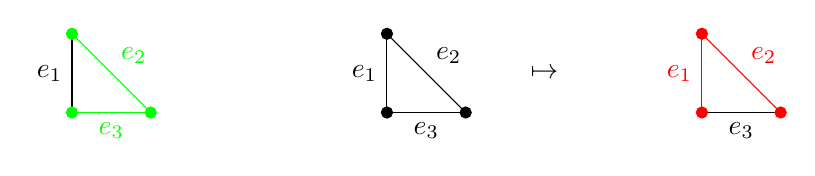
\begin{tikzpicture}

    \begin{scope}[xshift = -4 cm]
        
        \coordinate (v_1) at (0, 0);
        \coordinate (v_2) at (1, 0);
        \coordinate (v_3) at (0, 1);

        \draw [color = green] (v_1) -- node [below]       {$e_3$} (v_2);
        \draw [color = green] (v_2) -- node [above right] {$e_2$} (v_3);
        \draw [color = black] (v_3) -- node [left]        {$e_1$} (v_1);

        \filldraw [color = green] (v_1) circle (2pt);
        \filldraw [color = green] (v_2) circle (2pt);
        \filldraw [color = green] (v_3) circle (2pt);

    \end{scope}

    \draw (-2, 0.5) node {$\mapsfrom$};

    \begin{scope}
        
        \coordinate (v_1) at (0, 0);
        \coordinate (v_2) at (1, 0);
        \coordinate (v_3) at (0, 1);

        \draw [color = black] (v_1) -- node [below]       {$e_3$} (v_2);
        \draw [color = black] (v_2) -- node [above right] {$e_2$} (v_3);
        \draw [color = black] (v_3) -- node [left]        {$e_1$} (v_1);

        \filldraw [color = black] (v_1) circle (2pt);
        \filldraw [color = black] (v_2) circle (2pt);
        \filldraw [color = black] (v_3) circle (2pt);

    \end{scope}

    \draw (2, 0.5) node {$\mapsto$};

    \begin{scope}[xshift = 4 cm]
        
        \coordinate (v_1) at (0, 0);
        \coordinate (v_2) at (1, 0);
        \coordinate (v_3) at (0, 1);

        \draw [color = black] (v_1) -- node [below]       {$e_3$} (v_2);
        \draw [color = red]   (v_2) -- node [above right] {$e_2$} (v_3);
        \draw [color = red]   (v_3) -- node [left]        {$e_1$} (v_1);

        \filldraw [color = red] (v_1) circle (2pt);
        \filldraw [color = red] (v_2) circle (2pt);
        \filldraw [color = red] (v_3) circle (2pt);

    \end{scope}

\end{tikzpicture}
    \end{center}

    Der linke (grüne) Spannbaum hat $B_\mathrm{l}$ geringere Kosten als der rechte (rote) $B_\mathrm{r}$.

    \begin{align*}
        c(B_\mathrm{l})
        =
        c(e_2) + c(e_3)
        <
        c(e_1) + c(e_2)
        =
        c(B_\mathrm{r})
    \end{align*}

    \item Sei $E = [e_1, \dots, e_n]$ eine beliebige Kanten-Reihenfolge.
    Der gegebene Algorithmus operiert wie folgt.

    \begin{align*}
        E_0 := \emptyset,
        \quad
        E_{i+1}
        :=
        \begin{cases}
            (E_i \cup \Bbraces{e_{i+1}}) \setminus \Bbraces{e_{i_1}},
            &
            \Exists (e_{i_1}, \dots, e_{i_k}) ~\text{Zyklus}~ \subset (V, E_i \cup \Bbraces{e_{i+1}}): \\
            &
            c(e_{i_1}) \geq c(e_{i_2}), \dots, c(e_{i_k}), \\
            E_i \cup \Bbraces{e_{i+1}}, & \text{sonst}
        \end{cases}
    \end{align*}

    Der Algorithmus antwortet mit $(V, E_n)$.

    Um die Korrektheit des Algorithmus zu beweisen, brauchen wir zunächst ein Lemma.

    \textbf{Lemma.}
    Sei $G = (V, E)$ ein endlicher, zyklenfreier Graph.
    Sei $e$ eine Kante, sodass $G^\prime = (V, E \cup \Bbraces{e})$ einen Zyklus enthält.
    Dann enthält $G^\prime$ höchstens (d.h. genau) einen Zyklus.

    \textit{Beweis.}
    Angenommen, $G^\prime$ enthielte $2$ verschiedene Zyklen $a = (a_1, \dots, a_n)$ und $b = (b_1, \dots, b_m)$.
    Offenbar muss $e \in a$, da sonst $a$ Zyklus von $G$ wäre.
    Dasselbe gilt für $b \ni e$.
    Nun können wir aber aus $a \setminus e$ und $b \setminus e$ einen Zyklus von $G$ erzeugen.
    Widerspruch!

    Q.E.D.

    \textbf{Bemerkung.}
    Wenn man aus einem Graphen (z.B. $G^\prime$ aus dem obigen Lemma), der genau einen Zyklus besitzt eine Zyklus-Kante löscht, dann ist der resultierende Graph zyklenfrei.

    \textit{Beweis (Korrektheit von Maybe-MST-C).}
    Laut dem obigen Lemma und der Bemerkung, ist klar, dass $B = (V, E_n)$ zyklenfrei ist.
    $B$ ist aber auch zusammenhängend:

    Sei $i = 1, \dots, n$ und verbinde $e_{i+1}$ zwei Zusammenhangskomponenten $Z_1, Z_2 \subseteq (V, E_i)$.
    Wir behaupten, dass $(V, E_i \cup \Bbraces{e_{i+1}})$ zyklenfrei ist.
    Laut dem obigen Lemma und der Bemerkung, ist nämlich klar, dass $(V, E_i)$ zyklenfrei ist.
    Daher sind insbesondere die Zusammenhangskomponenten (Bäume) $Z_1$ und $Z_2$ zyklenfrei.
    $Z := Z_1 \cup \Bbraces{e_i} \cup Z_2 \subseteq (V, E_i \cup \Bbraces{e_{i+1}})$ ist also auch zyklenfrei.
    $(V, E_i \cup \Bbraces{e_{i+1}})$ ist also insgesamt Zyklenfrei.
    Der Algorithmus entscheidet sich also für $E_{i+1} = E_i \cup \Bbraces{e_{i+1}}$.
    Zusammenfassend:
    Wenn $e_{i+1}$ zwei Zusammenhangskomponenten verbindet wird $e_{i+1}$ vom Algorithmus nicht entfernt.

    Wir zeigen mit Induktion, dass es immer, d.h. im $i$-ten Schritt, genug Kanten $\in \Bbraces{e_i, \dots, e_n}$ gibt, sodass alle Zusammenhangskomponenten von $(V, E_{i-1})$ verbunden werden können.
    Der Induktionsanfang ist klar, weil $G = (V, E)$ zusammenhängend ist und die Zusammenhangskomponenten von $(V, E_0)$ genau die Singleton-Graphen $(\Bbraces{v}, \emptyset)$, $v \in V$ sind.
    Für den Induktionsschritt gebe es solche Kanten im $i$-ten Schritt.
    Wenn keine der Kanten darin verwendet wurde, gibt es alle davon auch im $(i+1)$-ten Schritt wieder.
    Wenn eine ($e_i$) verwendet wurde, dann wurde sie laut den oberen Überlegungen nicht vom Algorithmus aus $E_i \cup \Bbraces{e_i}$ entfernt.
    Weil dann aber gerade zwei Zusammenhangskomponenten von $(V, E_{i-1})$ verbunden wurde, gibt es in $(V, E_i)$ dann aber genau eine Zusammenhangskomponente weniger.
    Die im $i$-ten Schritt verwendete Kante $e_i$ wird daher im $(i+1)$-ten (bis $n$-ten) Schritt garnicht mehr gebraucht, um diese Bereiche im Graphen zu verbinden, weil sie ja bereits, vermöge $e_i$ zusammenhängen.

    Der Algorithmus arbeitet alle Kanten $\in E$ ab, also auch all jene, die Zusammenhangskomponenten verbinden.
    Der resultierende Graph $B$ ist daher zusammenhängend.

\end{enumerate}

\end{solution}

% --------------------------------------------------------------------------------
